\section*{Problem No.2} \label{sec:prob2}
The following code implements Newton's method with optional Line Search 

\begin{lstlisting}
function [normF,X] = Newton(Func, Jac, X0, MaxIt, LS)   
    %apply Newton method and return the function norm for each iteration 
    %along with the step 
    %@Func is the input function(s) for which we are seeking the roots    
    %@Jac is a function to evaluate the Jacobian inverse for Func    
    %@X0 is the initial guess     
    %@MaxIt is the max number of iterations     
    %@LS is a flag to use line search     
    
    x = X0;
    X = X0';
    normF=norm(double(Func(x)));
    n = 1;
    tol = 1e-6;%stopping tolerance 
    while n < MaxIt %don't go beyound iteration limit 
        xn = x- Jac(x)*Func(x);
        X = [X;xn'];
        while LS && norm(Func(xn)) > norm(Func(x))
             %if we are overshooting and Line Search 
             x = (x+xn)/2.0;
             xn = x- double(Jac(x))*double(Func(x));
        end
        normF(end+1) = norm(double(Func(xn)));               
        if abs(normF(end)) < tol || abs(norm(X(end)) - norm(X(end-1))) <tol
            %stopping criteria on the size of the norm and step size 
            break;
        end
        x = xn; %swap for next iteration  
        n=n+1;
    end
end
\end{lstlisting}

The following tables shows the norm of $f$ for different steps for all the given initial guesses. We set the maximum iterations to 10. 

\begin{figure}[tbh]
 \centering
\begin{tabular}{ |c || c|c || c|c ||   c|c|}
 \hline
 \# Iteration  &\multicolumn{2}{|c||}{$x_{0}=(1,1)$} & \multicolumn{2}{|c||}{$x_{0}=(3,3)$} & \multicolumn{2}{|c|}{ $x_{0}=(10,10)$}\\ 
  \hline
 	& without LS & with LS & without LS & with LS & without LS & with LS\\
  \hhline{|=|=|=|=|=|=|=|}  
 1  &4.24264068	&4.24264068 &0.471404520 &0.471404520 &1.24783549 &1.24783549 \\
   \hline                                                                    
 2  &2.54558441	&2.54558441 &0.471404520 &0.471404520 &1.43981018 &1.41659784 \\
   \hline                                                                    
 3  &1.76232767	&1.76232767 &            &            &1.41466066 &1.41421756 \\
   \hline                                                                    
 4  &1.47163444	&1.47163444 &            &            &1.41421370 &1.41421356 \\
   \hline                                                                    
 5  &1.41636989	&1.41636989 &            &            &1.41421356 &1.41421356 \\
   \hline                                            
 6  &1.41421684	&1.41421684 &            &            &           &          \\
   \hline                                                                    
 7  &1.41421356	&1.41421356 &            &            &           &          \\
   \hline                                                                    
 8  &1.41421356  &1.41421356 &            &            &           &          \\
   \hline
\end{tabular} 
  \caption{The norm of $f$ for each iteration with and without Line Search for three initial guesses for the problem in part \emph{a}.}
   \label{tab:part_a}
\end{figure} 


\begin{figure}[tbh]
 \centering
\begin{tabular}{ |c || c|c || c|c |}
 \hline
 \# Iteration  &\multicolumn{2}{|c||}{$x_{0}=(1)$} & \multicolumn{2}{|c|}{$x_{0}=(10)$} \\ 
  \hline
 	& without LS & with LS & without LS & with LS\\
  \hhline{|=|=|=|=|=|}                           
1 &0.5		      & 0.5		     &0.9	   &0.9\\
\hline
3 & 0		      & 0    	     &1	       &1\\                                                                  
\hline
4 & 		      &     	     &1	       &1\\                                                                  
\hline
5 & 		      &     	     &1	       &NaN\\                                                                  
\hline
6 & 		      &     	     &1	       &NaN\\                                                                  
\hline
7 & 		      &     	     &1	       &NaN\\                                                                  
\hline
8 & 		      &     	     &NaN      &NaN\\
\hline
\end{tabular} 
  \caption{The norm of $f$ for each iteration with and without Line Search for three initial guesses for the problem in part \emph{b}.}
   \label{tab:part_b}
\end{figure} 




\begin{figure}[tbh]
 \centering
\begin{tabular}{ |c || c|c || c|c |}
 \hline
 \# Iteration  &\multicolumn{2}{|c||}{$x_{0}=(-1,-1)$} & \multicolumn{2}{|c|}{$x_{0}=(1,1)$} \\ 
  \hline
 	& without LS & with LS & without LS & with LS\\
  \hhline{|=|=|=|=|=|}                           
1 &5.65685424		      &5.65685424		     &10	       &10	 \\
    \hline                                                                    
2 &26.5658741 		      &0.315477033			&6.174254385   &6.1742543	\\
    \hline                                                               
3 &6.67111365		      &0.0055905271			&362.8979654   &24.159941	\\
    \hline                                                               
4 &1.14963256		      &1.7825251e-06	  	&93.89830153   &11.546005	\\
    \hline                                                               
5 &0.0642719172		  	  &1.7944114e-13  		&28.94233456   &0.63406588	\\
    \hline                                                               
6 &0.00023480631		      &                     &8.725054628   &0.13232260	\\
    \hline                                                               
7 &3.10261921e-09		  &                     &314474.5892   &0.0002253  \\
    \hline                                                               
8 &7.53374354e-16    	  &                     &93132.07088   &1.0477183e-08 \\
    \hline                                                               
9 &                        &                     &27560.41329   &0 \\
    \hline                                                               
10 &                        &                     &8138.148664   & \\
   \hline                                                                    
\end{tabular} 
  \caption{The norm of $f$ for each iteration with and without Line Search for three initial guesses for the problem in part \emph{c}.}
   \label{tab:part_c}
\end{figure} 


\paragraph{Comment of the results:}
For the first problem, the function is discontinuous as shown in Figure \ref{fig:fig_a}. That is why when we start with an initial guess that is far from the solution, the method fails even when using Line Search. 

For the third problem, the function has two solution as shown in Figure \ref{fig:fig_c}. Depending on the initial guess, the solution we get differ. The Line Search helped converging to the solution faster in both cases as the step history shows in Figure \ref{fig:fig_c}. 


\begin{figure}[wtbh]
 \centering  
   {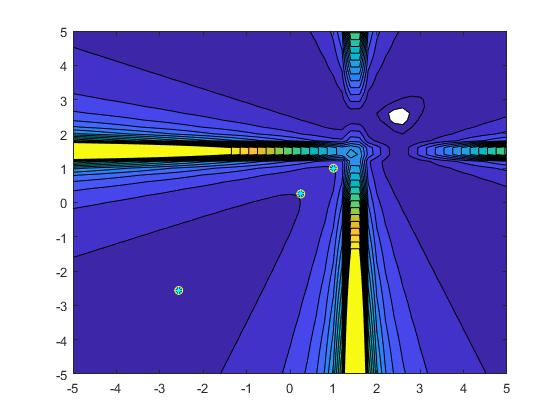
\includegraphics[width=0.49\linewidth]{fun1_a1.jpg}}   
   {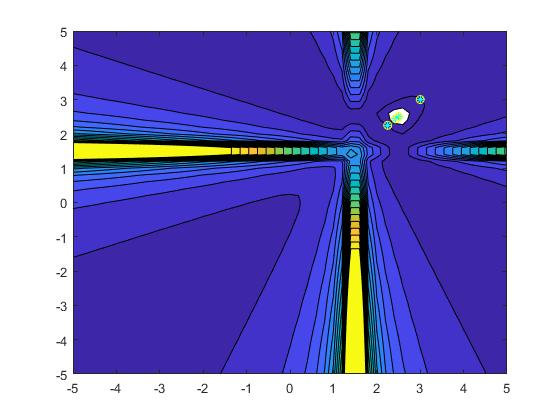
\includegraphics[width=0.49\linewidth]{fun1_a2.jpg}}
  \caption{Contours of $||f||$ as a function of $x_{1}$ (x-axis) and $x_{2}$ (y-axis) for initial guess $(1,1)$ (left) and $(3,3)$ (right) for the problem in part \emph{a}. The solution after each iteration is plotted as star for when Line Search is not used and empty circle when it is used. Both solution coincide.}
   \label{fig:fig_a}
\end{figure} 


\begin{figure}[tbh]
 \centering  
   {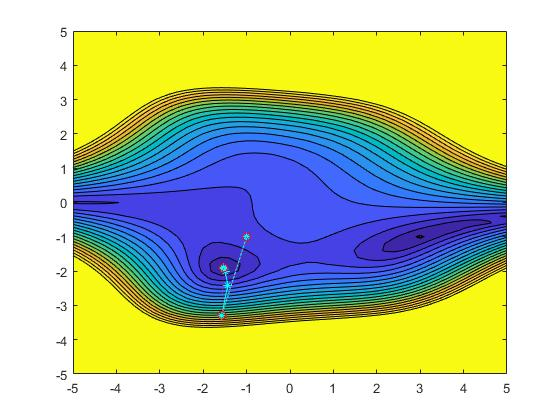
\includegraphics[width=0.49\linewidth]{fun3_a1.jpg}}   
   {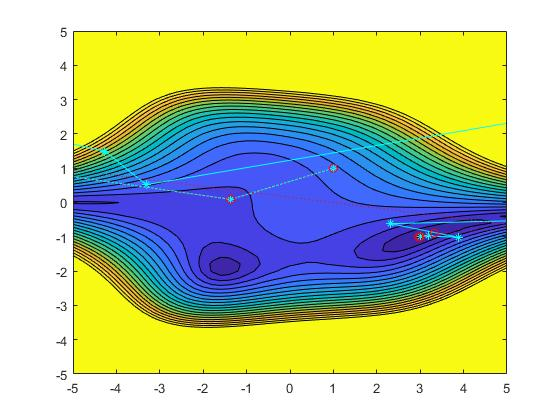
\includegraphics[width=0.49\linewidth]{fun3_a2.jpg}}
  \caption{Contours of $||f||$ as a function of $x_{1}$ (x-axis) and $x_{2}$ (y-axis) for initial guess $(-1,-1)$ (left) and $(1,1)$ (right) for the problem in part \emph{c}. The solution at each step is shown as solid line when no Line Search is used and dotted for Line Search.}
   \label{fig:fig_c}
\end{figure} 